\section{Overview}

This thesis is concerned with solving one of the principal problems in the field of planet formation, how can we detect newly-formed planets, and measure their properties?
Answering this question is a vital step in constraining the various theoretical models of the planet formation process.

\begin{itemize}
    \item Explain briefly star and disk formation. Define circumstellar disk and protoplanetary disk.
    \item Explain briefly the properties of the disk. Define accretion disk.
    \item Explain briefly models of planet formation, define protoplanet.
\end{itemize}

%Important clues for how planets are formed around young stars can be found in the structure of our own Solar System, namely in the difference between the mass and angular momentum distributions. 
%The Sun contains $99.86 \%$ of the total mass in the Solar System, while the orbits of the planets contain $98.5 \%$ of the total angular momentum \citep[eg.][]{woolfson2000}.
%This segregation proved to be a significant challenge for early models of the formation of the Solar System, eventually culminating in the idea that the planets must have formed from a vast disk of gas and dust surrounding the Sun \citep[see review by][]{edgeworth1949}.

%The birthplace of stars and planets are large interstellar clouds composed primarily of hydrogen gas, known as molecular clouds \citep[e.g.][]{larson2003}, which have typical sizes of $2$ -- $15$ $\rm{pc}$ and masses of $10^3$ -- $10^5$ $\rm{M_\odot}$ \citep{cambresy1999}. 
%Before observational advances made in the past 30-40 years, our understanding of how stars and planets form in these clouds was essentially as follows.
%The molecular cloud gradually collapses under its own gravity, resulting in the formation of overdense clumps \citep{norman1980}.
%Continued collapse causes these dense regions of the cloud to become unstable to their self-gravity, leading to the fragmentation of the cloud and the formation of stellar cores \citep{jeans1902,larson1969,penston1969,shu1977}. 
%During the collapse, conservation of angular momentum results in the formation of an accretion disk around the protostar \citep{terebey1984,shu1987}.
%Centripetal acceleration resists further collapse against gravity in the disk plane, while collapse in the perpendicular direction proceeds basically unimpeded resulting in vertical hydrostatic equilibrium \citep{pringle1981}.
%The resultant circumstellar disk, known at this stage of evolution as a protoplanetary disk, is then the site of planet formation.

\section{Protoplanet Detection}



\begin{figure}[H]
    \centering
    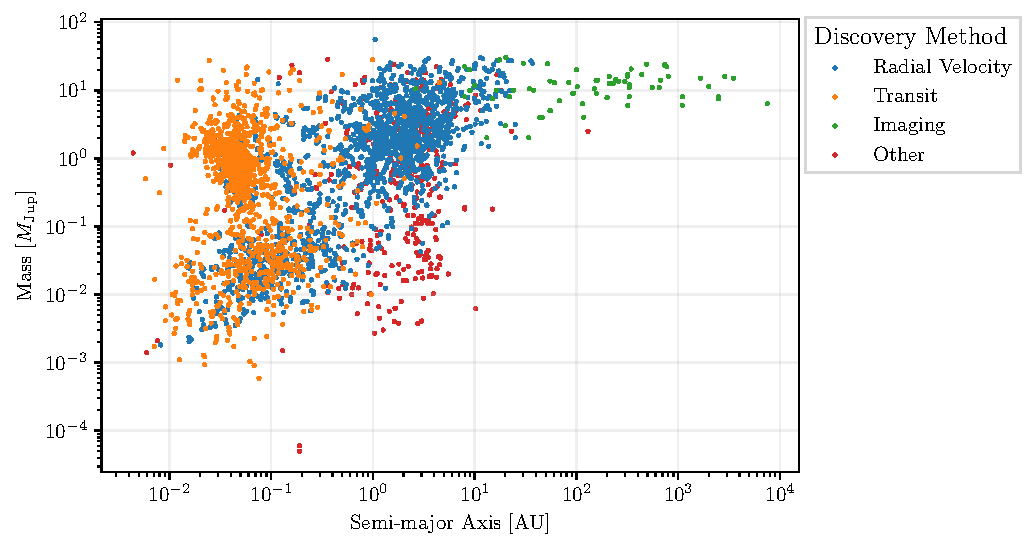
\includegraphics[width = 0.98\textwidth]{figures/exoplanet.pdf}
    \caption{}
    %Planet-mass and semi-major axis plotted for all confirmed exoplanets and candidate protoplanets. Grey dots represent exoplanets detected through traditional means and the black squares represent the planets of the solar system. The coloured symbols all represent candidate planets detected through disk substructures, green spirals for spiral structures and blue dots for ring structures, or through kinematic signatures shown by the red lightning symbols. Plotted also are the regions of parameter space that each exoplanet detection method may probe \citep{diskdynamicscollaboration2020}.
    \label{fig:exoplanets}
\end{figure}

%The first exoplanet was discovered in 1995 and was unlike anything found in the solar system.
%51 Pegasi b is a ``hot Jupiter'', with a mass around half that of Jupiter, but completing its orbit in only 4 days.
%This places it nearly 20 times closer to its star than the Sun is to the Earth \citep{mayor1995}. 
%In the nearly 30 years since that landmark discovery the number of confirmed exoplanets has skyrocketed to 5044 \citep{nasa2022}.
%The mass and orbital radius distribution of these planets is shown in Figure \ref{fig:exoplanets}.
%Despite this success, the number of uncontroversially confirmed planets found still in the process of forming, called protoplanets, sits at an unimpressive total of two, both around PDS 70 \citep{keppler2018,haffert2019}, and observed through direct imaging in the near-infrared.
%This lack of protoplanet detections is primarily because the most successful methods of exoplanet detection are unviable in the environment found around stars with ages up to a few Myr \citep{luhman2010}.
%This environment consists of a vast disk of gas, primarily $\mathrm{H_2}$, and dust, surrounding the star \citep[eg.][]{armitage2010}.
%Such disks are known as circumstellar disks, and those found around young stars are called protoplanetary disks.
%
%By far the most common exoplanet search methods are the transit method and radial velocity methods, with 3864 and 930 confirmed detections respectively.
%The transit method, which relies on periodic dimming of the star's light from an obstructing planet, is hindered by the presence of optically thick material in the disk plane (although one has been found in the optically thin dust disk surrounding K2-33, see \citet{david2016}).
%Moreover, radial velocity searches are made difficult by the high starspot and accretion activity of young stars, which makes disentangling possible signals of planets present in spectra very challenging \citep{desort2007}.
%While there are three candidate detections for exoplanets in orbit around around V830 Tau \citep{donati2015} CI Tau \citep{johns-krull2016} and TAP 26 \citep{yu2017}, both TAP 26 and V830 Tau are weak-line T Tauri stars whose disks have already dissipated, and the V830 Tau and CI Tau detections are disputed \citep{damasso2020,donati2020}.

%Detecting these hypothesised planets directly is a formidable task.
%The most successful exoplanet detection methods by number of detections, the radial velocity and transit methods, are both unviable due to the presence of disk material.
%Direct imaging on the other hand has seen some success, with two planets detected in the disk around PDS 70 \citep{keppler2018,haffert2019}.
%Additional detections have been claimed in the disks of HD 100546 \citep{quanz2013}, HD 169242 \citep{biller2014}, LkCa15 \citep{sallum2015} and MWC 758 \citep{reggiani2018}.
%However, each of these is disputed in the literature \citep{rameau2017,ligi2018,currie2019}.
%The main difficulty is the possible confusion of disk material with a planet, since processing techniques can create spurious point sources from filamentary structures like arcs and spirals \citep[eg.][]{rameau2017}.
%Recently a detection was claimed in the disk around AB Aurigae through direct imaging \citep{currie2022}.
%Figure \ref{fig:ABAur} shows an image of AB Aurigae taken with the CHARIS integral field spectrograph on the Subaru telescope.
%The green circle indicates the location of the proposed planet, clearly embedded in a large spiral structure.
%This and other proposed detections raise the question for images of disks: when is a clump a disk structure, and when is it a planet?

\section{Disk Substructures}

\begin{figure}
    \centering
    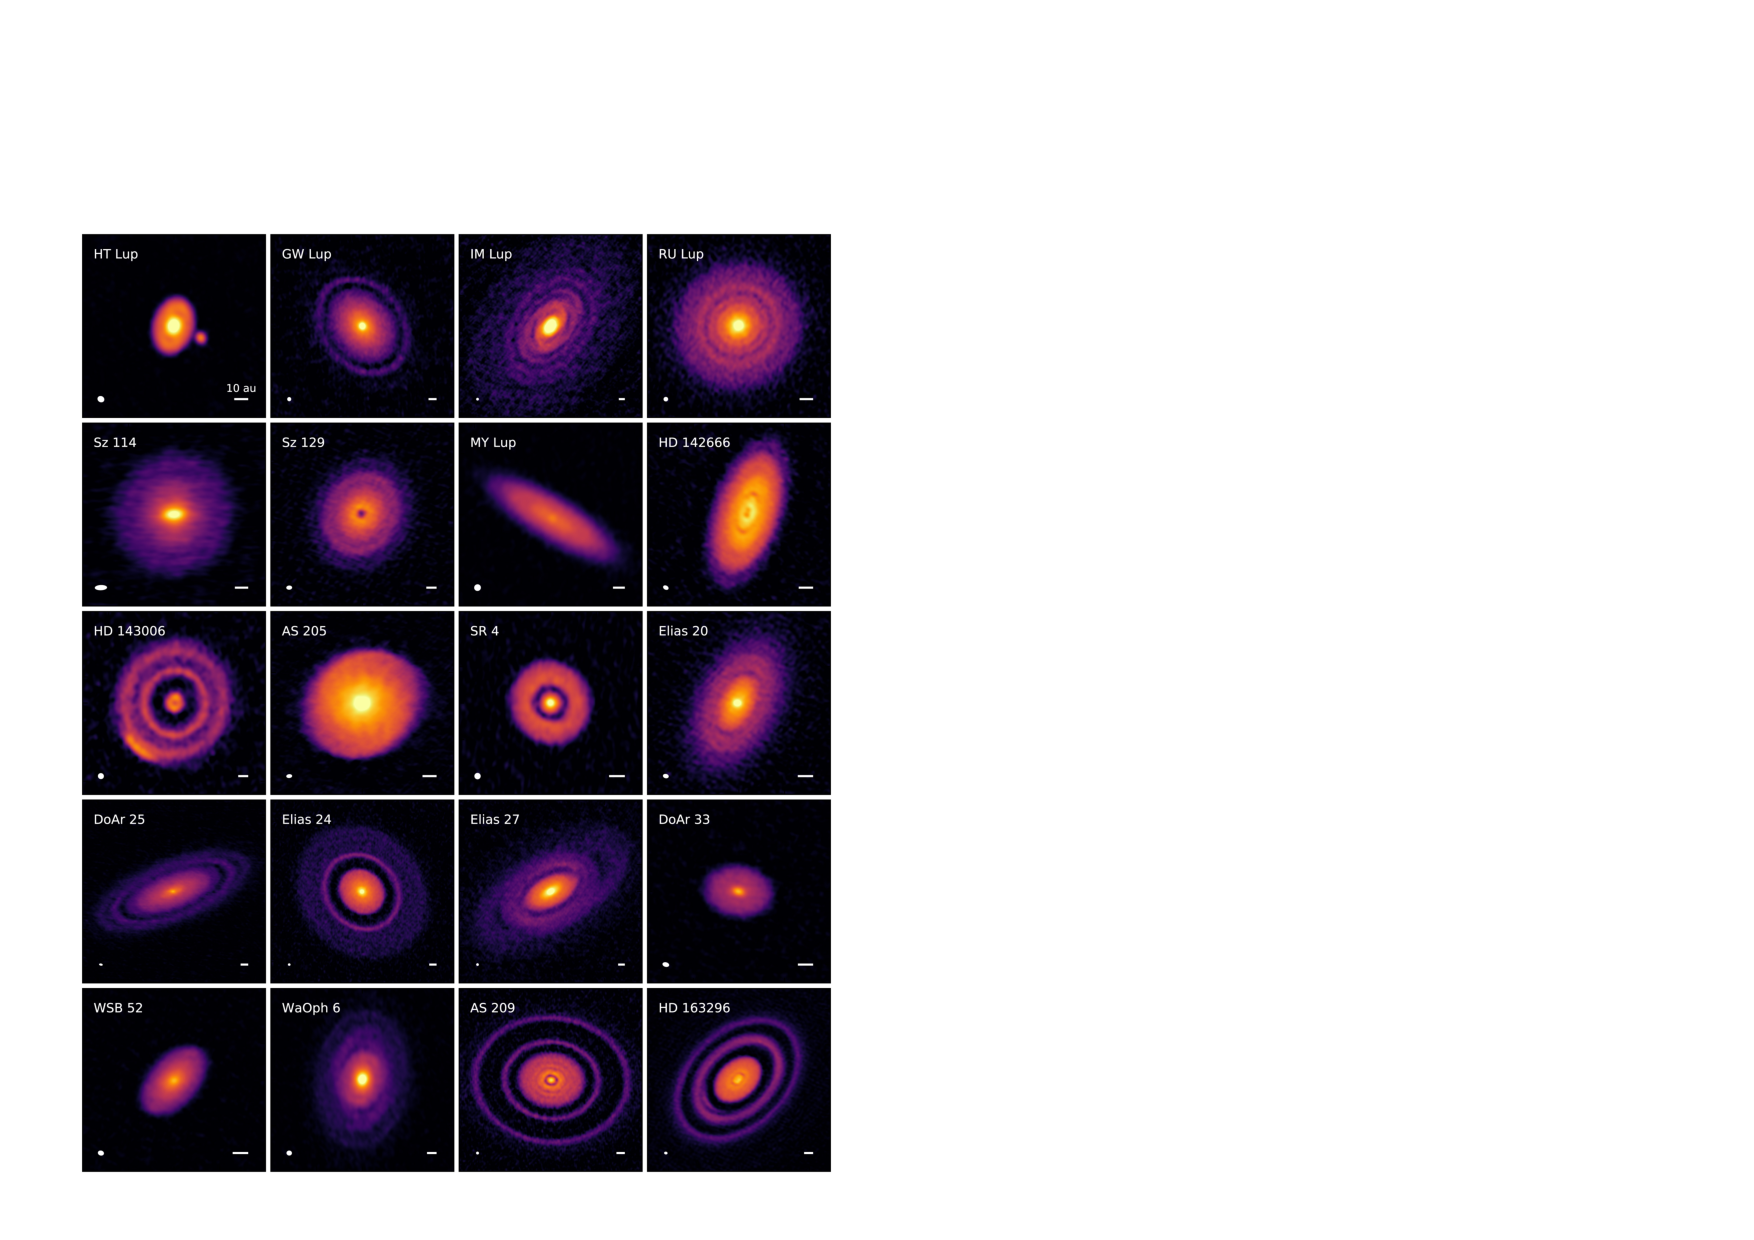
\includegraphics[width = 0.9\textwidth]{figures/DSHARP.pdf}
    \caption{Continuum images taken at 1.5 mm of the 20 protoplanetary disks in the DSHARP program. The colour scale has been stretched to increase the contrast. \citep{andrews2018}. Substructures are evident in each disk. Notable examples include: the thin and wide rings in AS 209 and HD 163296, spiral arms in IM Lup and Elias 2-27, and a bright arc in HD 143006.}
    \label{fig:DSHARP}
\end{figure}

%The abundant and diverse collection of substructures found in high resolution images of protoplanetary disks constitutes further evidence for early planet formation.
%Figure \ref{fig:DSHARP} shows continuum images taken as part of the Disk Substructures at High Angular Resolution Project (DSHARP) \citep{andrews2018}.
%All 20 of the disks exhibit some sort of substructure, including bright and dark rings, spiral arms and bright arcs.
%As we will discuss in section \ref{sec:interactions}, each of these features can be explained as arising from dynamical interactions between the disk and embedded protoplanets.
%
%Additional substructures in disks may be due to multiple star system interactions.
%It is clear that many stars form in binaries, with a disk around either each individual star or both together, with the latter known as a circumbinary disk \citep{white2001,akeson2014,akeson2019}.
%Observations show that many circumbinary disks have dark cavities where there is no emission, with the inner disk region presumably cleared of material from tidal interactions between the stars \citep{andrews2011}.
%Furthermore, disks have been observed containing misaligned inner disks, bridges and streams of material, all of which may be indicative of close encounters between stars and their disks \citep{dai2015,takami2018,rodriguez2018,cuello2019}.
%
%The evidence clearly does not support the picture of star and planet formation presented in sections \ref{sec:siteplanet} and \ref{sec:acc_disks}, where stars form individually, each star forms a disk, and later planets form in this disk. 
%Instead, it seems more likely that the process is significantly less ordered. 
%The modern understanding of star formation supports this picture.
%Many stars form together from local overdensities in the molecular cloud, caused by both gravitational contraction and turbulent flows \citep{larson1981,lada2003}.
%This environment is dynamic and chaotic, with many interactions between the newly formed stars. These interactions determine the properties of the resultant population \citep{bate2003,bate2012}.
%The disks that form within this environment are then subject to the same interactions.
%Figure \ref{fig:bate_disk_pop} shows 8 examples of disks formed in a large 3D hydrodynamical simulation with radiation, performed as part of a protostellar disk synthesis study by \citet{bate2018}.
%They find a diverse range of young disks; circumbinary disks, bridges between disks, misaligned disks, and disks with large spiral arms.
%If planets do form early and are already present in the protoplanetary stage, they must then begin forming soon after the disk has formed and the star is still embedded in its envelope as discussed in section \ref{sec:substructure}.
%
%Verifying these ideas relies on confirming that interactions between the disk and protoplanets are responsible for observed disk substructures, as alternative driving mechanisms have been suggested that do not involve planets.
%These include (but are not limited to): snow-lines \citep{kretke2007}, self-induced dust traps \citep{gonzalez2017} and the magnerotational instability \citep{simon2014}.

\section{Kinematic Observations}

\note{define ALMA, DSHARP and MAPS please. Also Jupiter mass, solar mass, Earth mass, moment maps, peak velocity, peak intensity.}

\begin{figure}
    \centering
    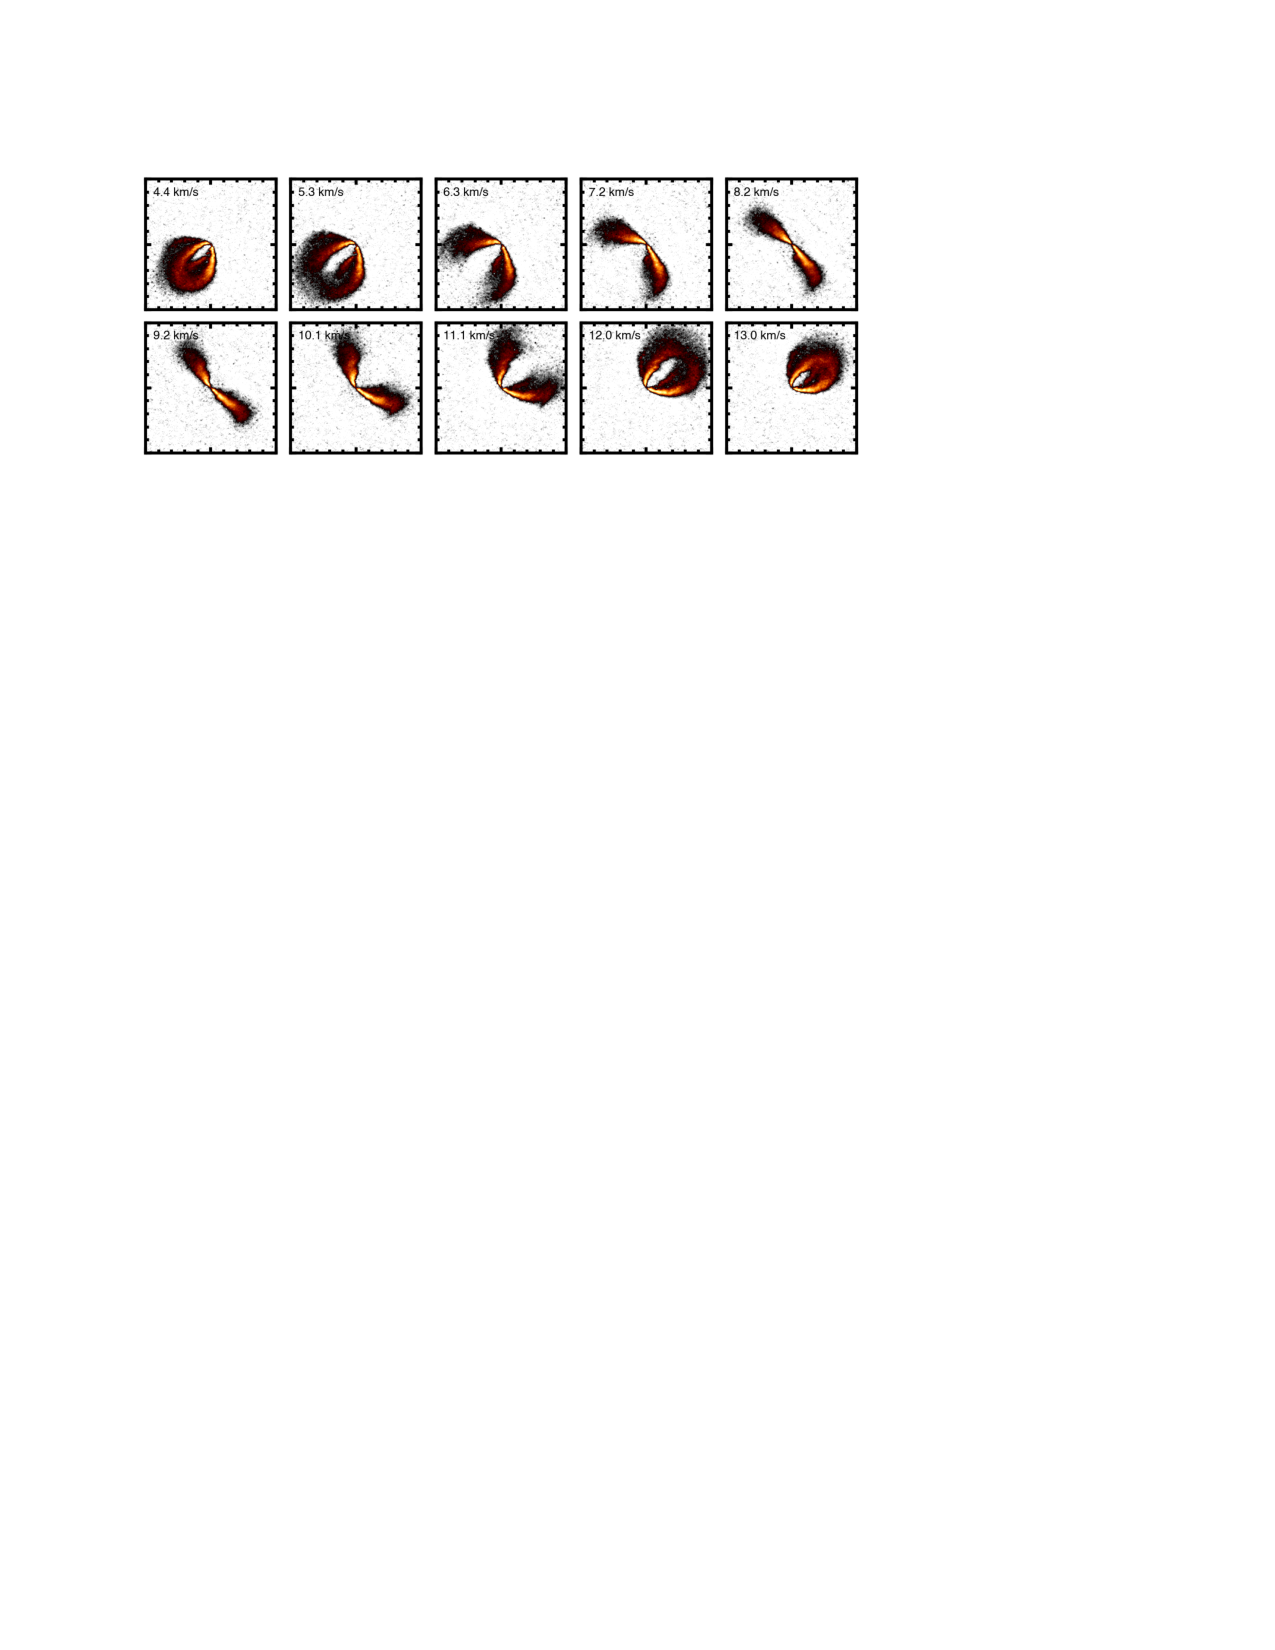
\includegraphics[width = 0.95\textwidth]{figures/channels.pdf}
    \caption{Velocity channels of $^{12}$CO emission from the disk around HD 163296 \citep{andrews2018}. The colour corresponds to brightness temperature, ie. brighter means more emission \citep{diskdynamicscollaboration2020}. Each channel probes the material in the disk moving at a certain velocity, resulting in the butterfly patterns seen across the channels. Note also that the CO emitting layer sits above the disk mid-plane, and so there is both a top and bottom surface in each image, with one surface mostly obscured by the other.}
    \label{fig:channels}
\end{figure}

\begin{figure}
    \centering
    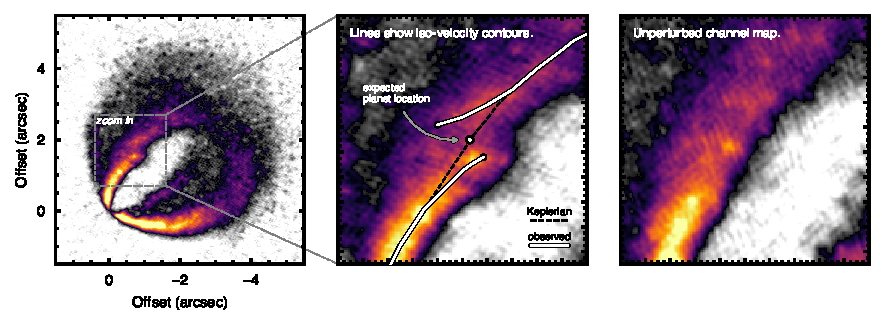
\includegraphics[width = 0.98\textwidth]{figures/HD163296_channels.pdf}
    \caption{A close view of 12 km/s velocity channel of HD 163296 \citep{andrews2018}, highlighting the velocity kink found by \citet{pinte2018a} Comparing the middle and right panels, we see how the line of maximum emission deviates from the iso-velocity contour expected from pure Keplerian rotation. \citep{diskdynamicscollaboration2020}.}
    \label{fig:velocity_kink}
\end{figure}

%Kinematic data from spectral line emission comes in the form of channel maps. 
%These are data cubes, with two spatial dimensions corresponding to the sky plane, and one frequency dimension.
%The frequency dimension is equivalent to velocity, and so in each frequency slice we find an image of all the material with the same line-of-sight velocity.
%Figure \ref{fig:channels} shows velocity channels of $^{12}$CO emission from HD 163296, imaged with ALMA \citep{andrews2018}.
%The observations show the expected butterfly shape that is characteristic of Keplerian rotation \citep{degregorio-monsalvo2013}.
%Note also that since $^{12}$CO line emission occurs at multiple scale heights, there is a top and bottom surface in each image.

%Since velocity channels probe the material moving at a certain line-of-sight velocity, the maximum emission in each channel should trace an iso-velocity contour.
%These iso-velocity contours are the lines of constant line-of-sight velocity, and they should be continuous and smoothly varying for Keplerian rotation.
%\citet{pinte2018a} found deviations from this smooth iso-velocity contour in ALMA data of the disk around HD 163296 \citep{degregorio-monsalvo2013,isella2016}, as pictured in Figure \ref{fig:velocity_kink}.
%This deviation has been dubbed a ``velocity kink'', and the authors found that it matched the expected signature that would be induced by a massive perturbing body as found by \citet{perez2015}.
%Numerical modelling showed that an embedded protoplanet of $3 - 5 \, M_\mathrm{J}$ (where $M_\mathrm{J}$ is a Jupiter mass) is able to accurately reproduce the observed channels. %, as shown in Figure \ref{fig:synthetic_channels} \citep{pinte2018a}.
%This is picture is supported by \citet{teague2018} who traced the gas pressure in the disk and found a best fit compatible with that found by \citep{pinte2018a}.
%\citet{pinte2019} also detected a velocity kink in CO observations of HD 97048, and used similar modelling to show that a planet of a few $M_\mathrm{J}$ is able to explain the observations.
%Importantly, the models for the embedded planets in both the HD 163296 and HD 97048 disks place the planet \textit{inside} observed dust gaps, providing strong evidence that the gaps are in fact carved by planets.
%Tentative detections of kinematic signatures have also been found in CI Tau \citep{rosotti2021} and 8 of 18 disks observed in the DSHARP program \citep{andrews2018,pinte2020}.
%The detections in the DSHARP disks all correspond to locations in a dust gap.

%Another piece of kinematic evidence for protoplanets is the ``doppler-flip'' that occurs across the planet location, due to the change in sign in the velocity perturbation \citep{perez2018a}. 
%\citet{casassus2019} and \citet{perez2020} found evidence for a doppler-flip in the disk of HD 100546, although they conclude that the induced deviations may be too large to be explained by a planet.